\subsection{Répartition des tâches}

\subsection{Outils utilisés}

\subsubsection{Gestionnaire de versions}
Tout au long du projet, nous avons utilisé \emph{git} : un gestionnaire de version décentralisé. Un tel outil permet la mise en commun des travaux, la gestion des versions et la gestion des \emph{merges}\footnote{Fusion de deux fichiers différents.}. 

\begin{figure}[H]
	\centering
	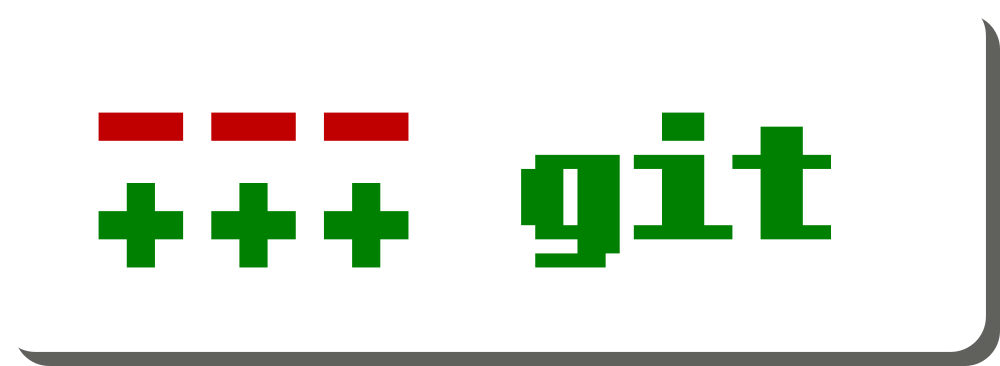
\includegraphics[width=0.3\textwidth]{files/outils/git}	
	\caption{Logo de \emph{git}}
	\label{git}
\end{figure}

Nous avons choisi \emph{git} pour plusieurs raisons :

\begin{itemize}
\item plutôt simple d'utilisation (par rapport à ses homologues comme \emph{SVN}),
\item hébergement gratuit via GitHub (sous condition de diffusion du code sous une licence libre),
\item \emph{git} est une solution libre sous licence \gls{GPLv2}.
\end{itemize}

\subsubsection{EtherPad, un éditeur de texte collaboratif}
\emph{EtherPad} se présente sous la forme d'un éditeur de texte léger permettant de faire un minimum de mise en page.

\begin{figure}[H]
	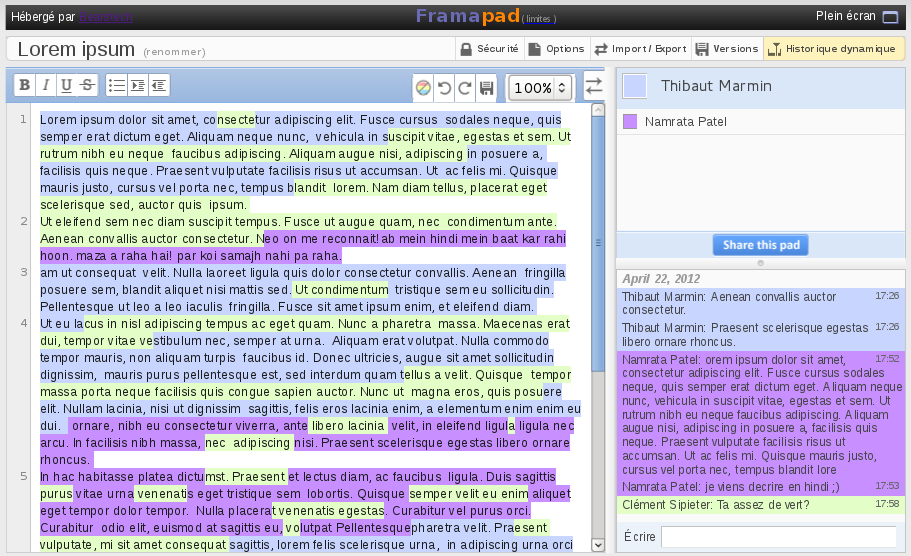
\includegraphics[width=\textwidth]{files/outils/etherpad_screenshot}	
	\caption{Aperçu de l'interface d'\emph{EtherPad} hébergé sur \emph{framapad} (site mis à disposition par Framasoft utilisant le code d'EtherPad).}
	\label{etherpad_screenshot}
\end{figure}

\begin{center}
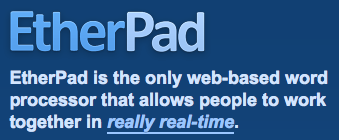
\includegraphics[width=0.4\textwidth]{files/outils/etherpad}
\end{center}


L'interface d'\emph{EtherPad} se présente sous la forme d'une interface web (figure \ref{etherpad_screenshot}) où chaque utilisateur connecté possède une couleur. La singularité de cet outil réside dans le fait que toutes les modifications effectuées sur le pad sont visibles par tous en temps réel.

Un chat est également disponible ce qui facilite la collaboration entre les utilisateurs connectés.

Il est important de noter qu'\emph{EtherPad} est sous licence \gls{Apache v2}.